\begin{frame}  
  \begin{figure}[h]
  	\begin{center}
      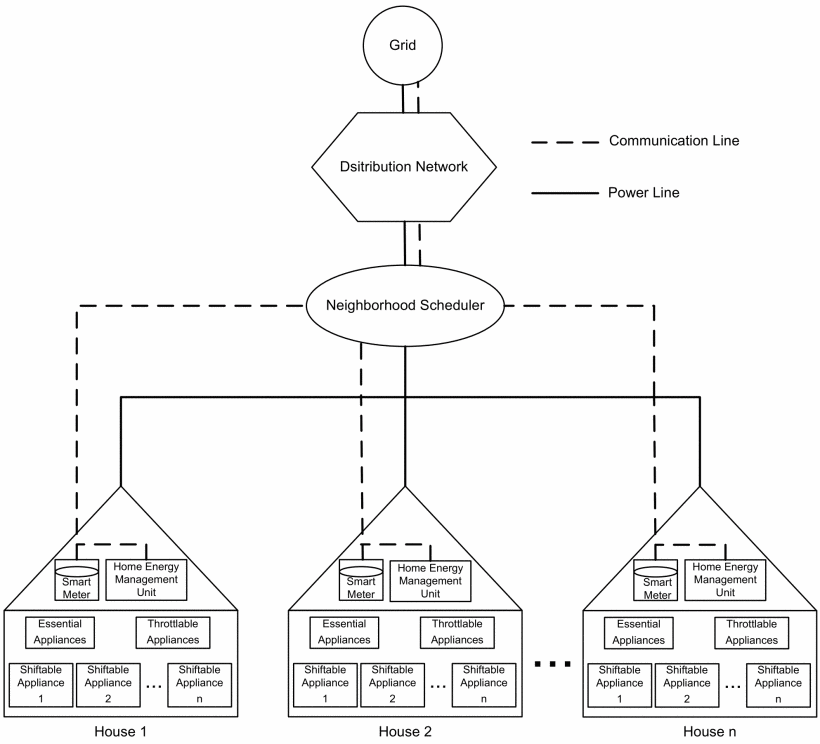
\includegraphics [scale=0.3]{./Figures/result1}
      \caption {Estrutura do sistema simulado e proposto}
  		%\label{fig:arq-imuno}
  	\end{center}
  \end{figure}
\end{frame}

\begin{frame}
  \begin{block}{}
    \begin{itemize}
      \item \alert{L1}, \alert{L2}, \alert{L3}, \alert{L4} e \alert{L5} respresentam as cargas deslocáveis dadas pelo consumidor
      \item Intervalos de demanda preferíveis informados pelo consumidor
      \item Valor ótimo gerado pelo algoritmo 
    \end{itemize}  
  \end{block}
  
  \begin{figure}[h]
  	\begin{center}
      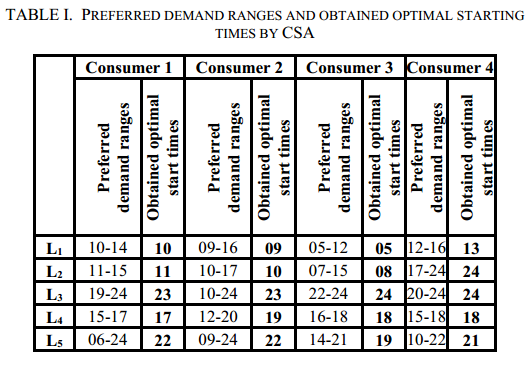
\includegraphics [scale=0.45]{./Figures/result2}
      \caption {\footnotesize Faixas de demandas preferidas pelo usuário e tempo de iniciação ótimo obtido pelo CSA}
  		%\label{fig:arq-imuno}
  	\end{center}
  \end{figure}
\end{frame}

\begin{frame}
  \begin{block}{}
    \begin{itemize}
      \item Os dados são aplicados ao \alert{AG} e ao \alert{CSA}
      \item Na figura é possível observar que o CSA se demonstrou mais eficiente que o AG (10 experimentos realizados)
      \item Melhores valores de fitness: 218.000 (AG) e 176.000 (CSA) 
    \end{itemize}
  \end{block}
  
  \begin{figure}[h]
  	\begin{center}
      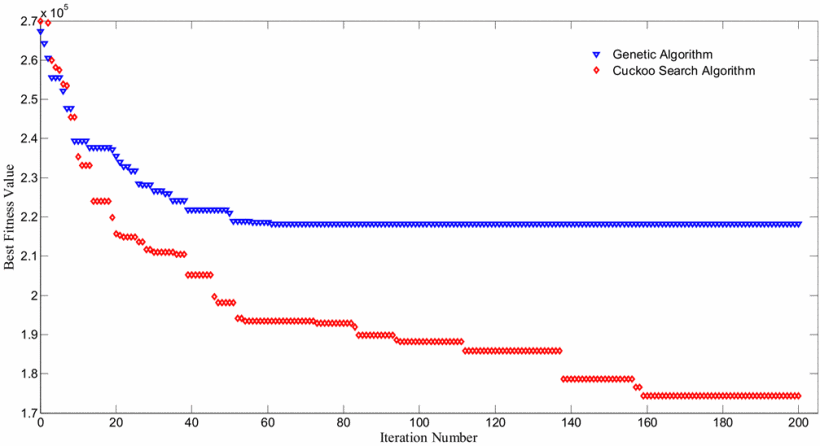
\includegraphics [scale=0.32]{./Figures/result3}
      \caption {Comparativo entre os resultados dos algoritmos de otimização}
  		%\label{fig:arq-imuno}
  	\end{center}
  \end{figure}
\end{frame}

\begin{frame}
  \begin{block}{}
    \begin{itemize}
      \item \small A redução da carga de pico é alcançada pelo escalonamento proposto
      \item \small \alert{O pico de carga é reduzido em 22\%}  
      \item \small A razão entre pico e média (PAR) diminuiu de 3,27 para 2,53 após o agendamento
    \end{itemize}
  \end{block}
  
  \begin{figure}[h]
  	\begin{center}
      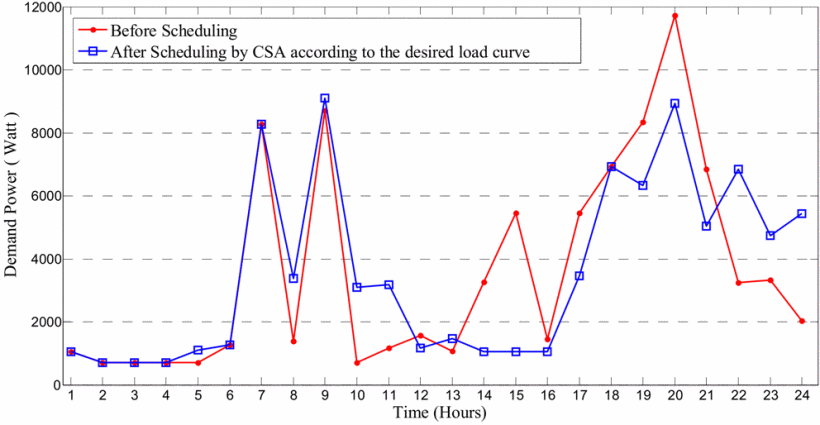
\includegraphics [scale=0.32]{./Figures/result4}
      \caption {Curvas de consumo agregado das casas}
  		%\label{fig:arq-imuno}
  	\end{center}
  \end{figure}
\end{frame}
%\begin{frame}
%  \begin{block}{}
%    \begin{itemize}
%      \item
%    \end{itemize}
%  \end{block}
%\end{frame}

%\begin{frame}
%  \begin{block}{}
%  \end{block}
%\end{frame}

%\begin{frame}
%  \begin{figure}[h]
%  	\begin{center}
%      \includegraphics [scale=0.3]{./Figures/Device-Estimates}
%     % \caption {Estimativa de dispositivos conectados à Internet.}
%  		%\label{fig:arq-imuno}
%  	\end{center}
%  \end{figure}
%\end{frame}

%\begin{frame}{Redes de Acesso}
%	\begin{figure}[!htb]
%		\centering
%		\subfloat[DSL]{
%			\includegraphics[height=3.5cm]{./Figures/DSLaccess}
%			\label{figdroopy}}
%		\quad %espaco separador
%		\subfloat[Cable]{
%			\includegraphics[height=3.5cm]{./Figures/CableAccess}
%			\label{figsnoop}}
%		%\caption{Subfiguras}
%		%\label{fig01}
%	\end{figure}
%\end{frame}

%\begin{frame}[fragile]
%\scriptsize
%\begin{verbatim}
%\end{verbatim}
%\end{frame}

%\begin{frame}{\textit{Socket Programming with TCP}}
%\scriptsize
%\lstinputlisting[language=Python, caption={TCP Server.}]{./code/upperServer/TCPserver.py}
%\end{frame}
